\chapter{Arrays}
\renewcommand{\chaptertitle}{Arrays}

\lehead[]{\normalfont\sffamily\hspace*{-2.00cm}\textcolor{white}{\colorbox{lightblue}{\makebox[1.60cm][r]{\thechapter}}}\hspace{0.17cm}\textcolor{lightblue}{\chaptertitle}}
\rohead[]{\textcolor{lightblue}{\chaptertitle}\normalfont\sffamily\hspace*{0.17cm}\textcolor{white}{\colorbox{lightblue}{\makebox[1.60cm][l]{\thechapter}}}\hspace{-2.00cm}}
%\chead[]{}
\rehead[]{\textcolor{lightblue}{AvHG, Inf, My}}
\lohead[]{\textcolor{lightblue}{AvHG, Inf, My}}

\lstset{style=myJava}

Zur Verwaltung großer Mengen von Daten gibt es sogenannte \emph{Arrays}
(Datenfelder). Mit einer einzigen Array-Variablen kann man ein ganzes Feld von
Daten eines Datentyps verwalten.

\begin{tcolorbox}[colback=blue!5,colframe=lightblue,boxrule=0.8pt,arc=3pt,title={\textbf{Hinweis zur Stoffauswahl in diesem Kapitel}}]
\small
Für den Pflichtteil dieses Kapitels genügen \textbf{eindimensionale Arrays}
(Abschnitt~19.1.1 und~19.2).\\
Der Abschnitt~19.1.2 (\emph{Mehrdimensionale Arrays}) ist nur dann
erforderlich, wenn ihr die weiterführenden LK-Übungsaufgaben
(\emph{Game of Life}, \emph{Mandelbrot-Menge} oder \emph{Clifford-Attraktor}) 
bearbeitet.\\
\textbf{Wichtig für den Leistungskurs:} Im Abschnitt~19.4 lernt ihr mit der
\myClass{ArrayList} eine deutlich flexiblere Alternative zu starren Arrays
kennen, die wir in Q2 (z.\,B.\ bei Netzwerk-Servern) wieder aufgreifen.
\end{tcolorbox}


\section{Arrays von primitiven Datentypen(boolean, int, double, char)}

\subsection{Eindimensionale Arrays \tagPflicht}

\subsubsection{Deklaration (Anlegen der Variablen)}

\begin{lstlisting}
int[] zahl;
boolean[] wahr;
\end{lstlisting}

\subsubsection{Erzeugung des Datenfeldes}

\begin{lstlisting}
zahl = new int[200];                æ// erzeugt ein Feld mit Index 0 bis 199
æwahr = new boolean[2];              æ// erzeugt ein Feld mit Index 0 bis 1
\end{lstlisting}

\subsubsection{Deklaration und Erzeugung gleichzeitig}

\begin{lstlisting}
int[] zahlen = new int[15];         æ// erzeugt 15 int-Zahlen
æint[] liste = {10,3,12,3,5};        æ// erzeugt ein Array mit 5 int-Zahlen
æboolean[] b = {true, true, false};  æ// erzeugt ein Array mit 3 boolean-Werten
\end{lstlisting}

\subsubsection{Verwendung des Datenfeldes (einfache Datentypen)}

Bei einfachen Datentypen wie \lstinline|int| oder \lstinline|boolean|,
kann man die erzeugten Feldelemente über den Index ansprechen und Werte
hinein schreiben:

\begin{lstlisting}
for (int i = 0; i < 200; i++) {
    zahl[i] = 10 + i;
}
wahr[0] = false;
wahr[1] = true;
\end{lstlisting}

\subsubsection{Übergabe eines Arrays an eine Methode}

Aufruf der Methode:

\begin{lstlisting}
int summe1 = addieren(zahlen);
int summe2 = addieren(liste);
\end{lstlisting}

Deklaration der Methode:

\begin{lstlisting}
public int addieren (int[] feld) {
// addiert alle Zahlen des Feldes und gibt die Summe zurück
    int summe = 0;
    for (int i = 0; i < feld.length; i++) {
        summe += feld[i];
    }
    return summe;
}
\end{lstlisting}

Der Parameter \lstinline|feld| ist ein Array vom Typ \lstinline|int| von
beliebiger Länge. Es wird die Speicheradresse des Arrays übergeben, so dass sich
Änderungen im Array durch die Methode auch auf die übergebene Array-Variable
auswirken!

Das im Schleifenkopf benutzte Attribut \lstinline|feld.length| gibt die Länge
des Arrays an.


\subsection{Mehrdimensionale Arrays \tagLK}

Beispiele:

\begin{lstlisting}
boolean[][] zweidimensional = new boolean[4][3];
zweidimensional[0][0] = true; 
zweidimensional[1][0] = false;
... 
zweidimensional[3][2] = false;

int[][][] dreidimensional = new int[20][3][4]; 
dreidimensional[19][2][3] = -97;
...
\end{lstlisting}


\section{Arrays von Objekten \tagLK}

\subsubsection{Deklaration}

\begin{lstlisting}
Auto[] a;               æ// Variable vom Typ einer Klasse "Auto"
\end{lstlisting}

Es wird ein Speicherplatz angelegt, der später die Speicheradresse des
Datenfeldes speichern soll:

\begin{minipage}{0.15\textwidth}
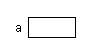
\includegraphics[width=1.0\textwidth]{./inf/SEKII/19_Java_Arrays/Deklaration.png}
\end{minipage}

\subsubsection{Erzeugung des Datenfeldes}

\begin{lstlisting}
a = new Auto[4];        æ// erzeugt Felder mit Index 0 bis 3
\end{lstlisting}

\begin{minipage}{0.45\textwidth}
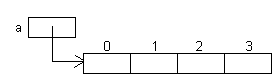
\includegraphics[width=1.0\textwidth]{./inf/SEKII/19_Java_Arrays/Erzeugung1.png}
\end{minipage}

\subsubsection{Erzeugung der Objekte}

Bei Feldern, die als Typ eine Klasse haben, muss man die einzelnen Objekte explizit erzeugen:

\begin{lstlisting}
a[0] = new Auto(10,20);
\end{lstlisting}

\begin{minipage}{0.45\textwidth}
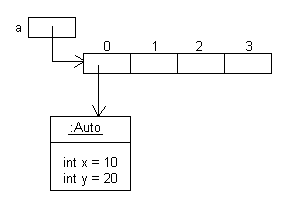
\includegraphics[width=1.0\textwidth]{./inf/SEKII/19_Java_Arrays/Erzeugung2.png}
\end{minipage}

Anschließend kann man Methoden und Variablen des Objektes aufrufen:

\begin{lstlisting}
a[0].x = 30;            æ// Verändert die Variable x des Objektes
æa[0].fahren(500);       æ// ruft die Methode "fahren" der Klasse Auto auf
\end{lstlisting}

%\pagebreak

In einer Schleife kann man alle Objekte des Feldes auf einmal erzeugen:

\begin{lstlisting}
for (int x = 0; x < a.length; x++) {
    a[x] = new Auto(x*10, 20);
}
\end{lstlisting}

\begin{minipage}{0.6\textwidth}
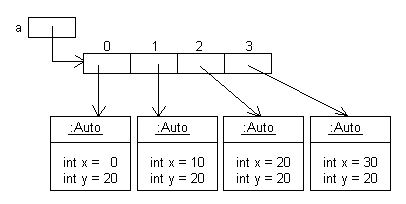
\includegraphics[width=1.0\textwidth]{./inf/SEKII/19_Java_Arrays/Erzeugung3.png}
\end{minipage}


\subsubsection{Die for-each Schleife (erweiterte for-Schleife) \tagZusatz \tagLK}

Wenn wir ein Array von Objekten – zum Beispiel ein Array \lstinline|hunde| vom Typ 
\lstinline|Hund[]| -- komplett durchlaufen wollen, haben wir bisher immer eine 
klassische Zählschleife verwendet:

\begin{lstlisting}
for (int i = 0; i < hunde.length; i++) {
    hunde[i].bellen();
}
\end{lstlisting}

Das funktioniert zwar zuverlässig, wirkt aber oft etwas umständlich: Eigentlich 
interessiert uns der Index \lstinline|i| hier gar nicht – wir wollen lediglich 
jedes einzelne Objekt im Array einmal ansprechen. Außerdem schleichen sich bei 
der Abbruchbedingung leicht Flüchtigkeitsfehler ein (etwa \lstinline|i <= hunde.length|, 
was sofort zu einer \lstinline|ArrayIndexOutOfBoundsException| führt).

Für genau solche Fälle bietet Java eine elegantere Schreibweise: die sogenannte 
\emph{for-each-Schleife} (im Englischen auch \emph{Enhanced for-Loop} genannt):

\begin{lstlisting}
for (Hund h : hunde) {
    h.bellen();
}
\end{lstlisting}

\textbf{So liest man die Schleife:}

Der Doppelpunkt : bedeutet hier so viel wie „in“ oder „aus“. Man liest die 
Kopfzeile also: „Für jedes Hund-Objekt \lstinline|h| in dem Array \lstinline|hunde|
führe den folgenden Anweisungsblock aus.“

Java kümmert sich im Hintergrund automatisch darum, dass das Array vom ersten 
bis zum letzten Element durchlaufen wird und die Schleifenvariable \lstinline|h| 
bei jedem Durchlauf auf das nächste Objekt im Array verweist.

\textbf{Wann nutzt man welche Schleife? (Wichtige Grenzen von for-each)}

Die for-each-Schleife macht deinen Quelltext deutlich kürzer und lesbarer, hat aber 
auch klare Einschränkungen. Du kannst sie nicht verwenden, wenn:

\begin{compactitem}
\item du den aktuellen Index \lstinline|i| benötigst (z.B.\ um auszugeben: 
„Hund Nr. 3 heißt Bello“ oder um zwei benachbarte Elemente wie \lstinline|zahlen[i]| und 
\lstinline|zahlen[i+1]| beim Sortieren zu vergleichen),
\item du das Array rückwärts oder nur teilweise durchlaufen möchtest,
\item du die Array-Einträge selbst ersetzen oder initialisieren möchtest 
(z.B.\ beim Befüllen eines leeren Objekt-Arrays mit \lstinline|new Hund(...)|, da 
eine Zuweisung an die lokale Hilfsvariable \lstinline|h| das eigentliche Array nicht 
verändert).
\end{compactitem}

\textbf{Faustregel für die Praxis:} Willst du alle Elemente eines Arrays einfach 
nur der Reihe nach auslesen oder auf ihnen Methoden aufrufen, ist die for-each-Schleife 
die erste Wahl. Sobald du Positionen (\lstinline|i|) vergleichen oder Array-Plätze neu 
belegen musst, greifst du zur klassischen for-Schleife.


\section{Dynamische Listen: Die Klasse \texttt{ArrayList} \tagLK}

Normale Arrays haben im Programmieralltag einen großen Nachteil: Man muss ihre
Größe bereits beim Erzeugen festlegen (\lstinline|new int[100]|). Wenn man
vorher nicht weiß, wie viele Elemente gespeichert werden sollen -- etwa wie viele
Clients sich gleich mit einem Chat-Server verbinden oder wie viele Treffer eine
Datenbankabfrage liefert --, sind Arrays unpraktisch.

Für solche Fälle bietet Java im Package \texttt{java.util} fertige
Sammlungen (\emph{Collections}) an. Die wichtigste Klasse für den Unterricht
ist die \myClass{ArrayList}: eine Liste, die beim Hinzufügen von Elementen
\textbf{automatisch wächst} und beim Löschen wieder schrumpft.


\subsection{Eine \texttt{ArrayList} anlegen und verwenden}

Beim Anlegen einer \myClass{ArrayList} gibt man in spitzen Klammern
(\texttt{<...>}, sogenannte \emph{Generics}) an, welchen Datentyp die Elemente
haben sollen:

\begin{lstlisting}
import java.util.ArrayList;

// Eine leere Liste für Zeichenketten anlegen:
ArrayList<String> namen = new ArrayList<>();

// Elemente hinzufügen (die Liste wächst automatisch):
namen.add("Anna");
namen.add("Ben");
namen.add("Clara");

// Auf ein einzelnes Element zugreifen (Index beginnt wie beim Array bei 0):
String ersterName = namen.get(0);   // liefert "Anna"

// Anzahl der gespeicherten Elemente abfragen:
int anzahl = namen.size();          // liefert 3

// Ein Element wieder entfernen (nachfolgende Elemente rücken auf):
namen.remove("Ben");                // oder über den Index: namen.remove(1);
\end{lstlisting}

\noindent \emph{Hinweis:} Die leeren spitzen Klammern \texttt{<>} auf der
rechten Seite (sogenannter \emph{Diamond-Operator}) von

\begin{lstlisting}
ArrayList<String> namen = new ArrayList<>();
\end{lstlisting}

sind eine Kurzschreibweise
für \lstinline|new ArrayList<String>()| -- Java übernimmt den Datentyp
automatisch von der linken Seite.

\begin{tcolorbox}[colback=orange!8,colframe=orange!80!black,boxrule=0.8pt,arc=3pt,title={\textbf{Wichtig bei Zahlen: Wrapper-Klassen verwenden!}}]
\small
In spitzen Klammern (\texttt{<...>}) erlaubt Java \textbf{keine primitiven
Datentypen} wie \lstinline|int| oder \lstinline|double|, sondern nur
Objekttypen (Klassen). Stattdessen nutzt man die passenden
\emph{Wrapper-Klassen}:
\begin{compactitem}
  \item \lstinline|ArrayList<Integer>| statt \lstinline|int|
  \item \lstinline|ArrayList<Double>| statt \lstinline|double|
  \item \lstinline|ArrayList<Boolean>| statt \lstinline|boolean|
\end{compactitem}
Das Umwandeln zwischen \lstinline|int| und \lstinline|Integer| übernimmt Java
beim Hinzufügen und Auslesen automatisch (\emph{Autoboxing}):\\
\lstinline|ArrayList<Integer> zahlen = new ArrayList<>();|\\
\lstinline|zahlen.add(42);| \quad \lstinline|int x = zahlen.get(0);|
\end{tcolorbox}


\subsection{Über alle Elemente einer Liste laufen (\texttt{for-each}-Schleife)}

Um alle Elemente einer \myClass{ArrayList} der Reihe nach zu verarbeiten, gibt
es neben der normalen Zählschleife (\lstinline|for (int i = 0; i < liste.size(); i++)|)
eine besonders kurze Schreibweise -- die sogenannte \emph{erweiterte
\texttt{for}-Schleife} (\texttt{for-each}):

\begin{lstlisting}
for (String aktuellerName : namen) {
    System.out.println("Hallo " + aktuellerName + "!");
}
\end{lstlisting}

\noindent \textbf{Lies den Doppelpunkt als \glqq aus\grqq :} \emph{\glqq Für
jeden \lstinline|String aktuellerName| aus der Liste \lstinline|namen| tue
Folgendes \ldots\grqq}


\subsection{Ausblick: Schlüssel-Wert-Paare mit \texttt{HashMap} \tagZusatz\tagLK}

Während eine \myClass{ArrayList} Elemente der Reihe nach über eine
Positionsnummer (\emph{Index} $0, 1, 2, \ldots$) verwaltet, braucht man in der
Praxis oft ein \glqq Nachschlagewerk\grqq : Man sucht einen Wert nicht über
seine Position, sondern über einen eindeutigen \textbf{Schlüssel} (\emph{Key})
-- etwa die Telefonnummer zu einem Namen, den Kontostand zu einer IBAN oder das
zugehörige \myClass{Socket}-Objekt zu einem Benutzernamen im Chat.

Dafür bietet Java die Klasse \myClass{HashMap} (ebenfalls aus dem Package
\texttt{java.util}). Sie speichert Paare aus \textbf{Schlüssel} (\emph{Key})
und \textbf{Wert} (\emph{Value}):

\begin{lstlisting}
import java.util.HashMap;

// Zuordnung von Name (Schlüssel: String) zu Punktzahl (Wert: Integer):
HashMap<String, Integer> punktestand = new HashMap<>();

// Einträge hinzufügen oder aktualisieren (put):
punktestand.put("Anna", 42);
punktestand.put("Ben", 37);
punktestand.put("Anna", 50);          // überschreibt Annas alten Wert!

// Wert über den Schlüssel gezielt abfragen (get):
int punkte = punktestand.get("Anna"); // liefert 50 (ohne Schleife!)

// Prüfen, ob ein Schlüssel vorhanden ist (containsKey):
if (punktestand.containsKey("Clara")) {
    System.out.println(punktestand.get("Clara"));
}

// Eintrag löschen (remove):
punktestand.remove("Ben");
\end{lstlisting}

\begin{compactitem}
  \item \textbf{Großer Vorteil:} Das Nachschlagen über \lstinline|get(schluessel)|
  funktioniert nahezu verzögerungsfrei, selbst wenn zehntausende Einträge
  gespeichert sind -- man muss nicht wie bei einer Liste alle Elemente in einer
  Schleife durchsuchen.
  \item \textbf{Wichtig:} Jeder Schlüssel darf in einer \myClass{HashMap} nur
  \textbf{einmal} vorkommen (ein erneutes \lstinline|put()| mit demselben
  Schlüssel überschreibt den bisherigen Wert), und es gibt keine feste
  Sortierreihenfolge.
\end{compactitem}



